\documentclass[11pt]{article}
\usepackage{amsmath,amsthm,amsfonts,amssymb,amscd}
\usepackage{multirow,booktabs}
\usepackage[table]{xcolor}
\usepackage{fullpage}
\usepackage{lastpage}
\usepackage{enumitem}
\usepackage{fancyhdr}
\usepackage{mathrsfs}
\usepackage{wrapfig}
\usepackage{setspace}
\usepackage{calc}
\usepackage{multicol}
\usepackage{cancel}
\usepackage[retainorgcmds]{IEEEtrantools}
\usepackage[margin=3cm]{geometry}
\usepackage{amsmath}
\newlength{\tabcont}
\setlength{\parindent}{0.0in}
\setlength{\parskip}{0.05in}
\usepackage{empheq}
\usepackage{framed}
\usepackage[most]{tcolorbox}
\usepackage{xcolor}
\usepackage{gensymb}
\colorlet{shadecolor}{orange!15}
\parindent 0in
\parskip 12pt
\geometry{margin=1in, headsep=0.25in}
\usepackage{tikz}

\newtheorem{clm}{Claim}

\title{Pursuit-Evasion in Graph Theory Research}
\author{Chancellor Lam}
\date{Summer 2024}

\begin{document}
	\maketitle
	\newpage
	\section{Franklin Graph}
	
	% define naming system for Franklin Graph vertices
	\begin{minipage}[c]{.45\textwidth}
		\centering
		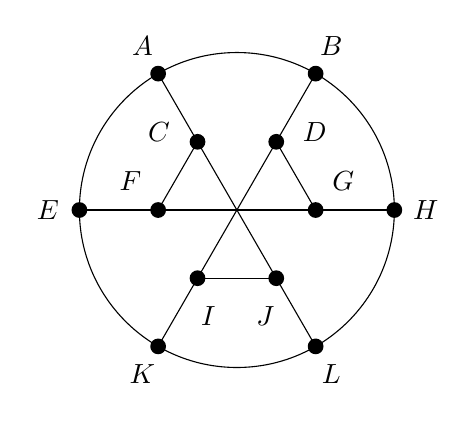
\begin{tikzpicture}[scale=2]
			\draw[white] (225:1.6) rectangle (45:1.6);
			\foreach \x/\y in
			{D/60, F/180, J/300}{
				\coordinate(\x) at (\y:0.5);
				\fill (\x) circle (0.5mm);
				\node at ({\y - 15}:0.7) {$\x$};
			}
			\foreach \x/\y in
			{C/120, G/0, I/240}{
				\coordinate(\x) at (\y:0.5);
				\fill (\x) circle (0.5mm);
				\node at ({\y + 15}:0.7) {$\x$};
			}
			
			
			\foreach \x/\y in
			{H/0, B/60, A/120, E/180, K/240, L/300}{
				\coordinate(\x) at (\y:1);
				\fill (\x) circle (0.5mm);
				\node at (\y:1.2){$\x$};
			}
			
			\foreach \x/\y in 
			{I/D,D/B,H/G,G/F,F/C,C/J,J/I,A/C,E/F,D/G,K/I,L/J}{
				\draw (\x)--(\y);
			}
			\draw circle (1);
		\end{tikzpicture}
	\end{minipage}
	\begin{minipage}[c]{.45\textwidth}
		\centering
		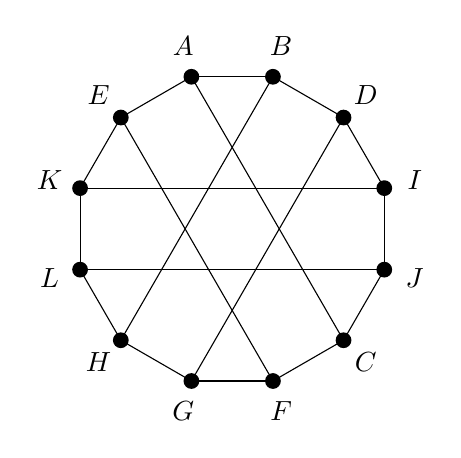
\begin{tikzpicture}[scale=2]
			\draw[white] (225:1.6) rectangle (45:1.6);
			\foreach \x/\y in {I/15,D/45,B/75,A/105,E/135,K/165,L/195,H/225,G/255,F/285,C/315,J/345}{
				\coordinate (\x) at (\y:1);
				\fill (\x) circle (0.5mm);
				\node at (\y:1.2) {$\x$};
			}
			
			\foreach \x/\y in {I/D,D/B,B/A,A/E,E/K,K/L,L/H,H/G,G/F,F/C,C/J,J/I,A/C,E/F,B/H,D/G,K/I,L/J}{
				\draw (\x)--(\y);
			}
		\end{tikzpicture}
	\end{minipage}
	
	% Claim 1
	\begin{clm}
		The metric dimension of the Franklin Graph is 4.
	\end{clm}
	\begin{proof}
		We will prove this by proving the following statements:
		\begin{enumerate}
			\item The metric dimension of the Franklin graph is less than or equal to 4.
			\item The metric dimension of the Franklin graph cannot be 3.
		\end{enumerate}
		We begin by proving that the metric dimension of the Franklin graph is less than or equal to 4. We will proceed by giving the chaser a strategy to win in one turn with 4 probes. The chaser should probe points $A,B,I,J$.
		\begin{center}
			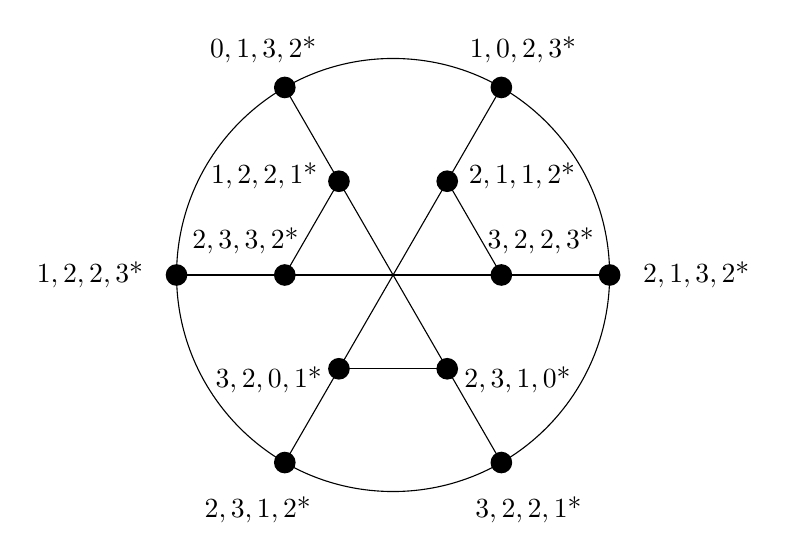
\begin{tikzpicture}[scale=2.75]
				\draw[white] (225:1.6) rectangle (45:1.6);
				\foreach \x/\y in
				{D/60, F/180, J/300}{
					\coordinate(\x) at (\y:0.5);
					\fill (\x) circle (0.5mm);
				}
				\foreach \x/\y in
				{C/120, G/0, I/240}{
					\coordinate(\x) at (\y:0.5);
					\fill (\x) circle (0.5mm);
				}
				
				
				\foreach \x/\y in
				{H/0, B/60, A/120, E/180, K/240, L/300}{
					\coordinate(\x) at (\y:1);
					\fill (\x) circle (0.5mm);
				}
				
				% inner ring (right)
				\node at (13:0.7){$3,2,2,3$*}; % G/0
				\node at (37.5:0.75){$2,1,1,2$*}; % D/60
				\node at (320:0.75){$2,3,1,0$*}; % J/300
				
				% inner ring (left)
				\node at (142.5:0.75){$1,2,2,1$*}; % C/135
				\node at (167:0.7){$2,3,3,2$*}; % F/180
				\node at (220:0.75){$3,2,0,1$*}; % I/225
				
				% outer ring
				\node at (0:1.4){$2,1,3,2$*}; % H/0
				\node at (120:1.2){$0,1,3,2$*}; % A/120
				\node at (60:1.2){$1,0,2,3$*}; % B/60
				\node at (180:1.4){$1,2,2,3$*}; % E/180
				\node at (240:1.25){$2,3,1,2$*}; % K/240
				\node at (300:1.25){$3,2,2,1$*}; % L/300
				
				\foreach \x/\y in 
				{I/D,D/B,H/G,G/F,F/C,C/J,J/I,A/C,E/F,D/G,K/I,L/J}{
					\draw (\x)--(\y);
				}
				\draw circle (1);
			\end{tikzpicture}
		\end{center}
		This will result in unique distances for all vertices. Since every vertex has a unique distance, it must be the case that the runner is located. Since it is the case that the chaser is able to locate the runner in 1 turn with 4 probes, it logically follows that the metric dimension of the Franklin graph is less than or equal to 4.
		
		We will now prove that the metric dimension of the Franklin graph cannot be 3. \\
		\textbf{*insert Reilly's Balanced Bipartite? theorem here to prove that the metric dimension of the Franklin graph cannot be 3 here* }
		
		Since the metric dimension of the Franklin graph is less than or equal to 4 and the metric dimension of the Franklin graph cannot be 3, it must be the case where the metric dimension is greater than 3 and less than or equal to 4.
		
		Therefore, the metric dimension of the Franklin graph is 4.
	\end{proof}
	
	% Claim 2
	\begin{clm}
		The Franklin Graph is locatable in 3 turns with 2 probes.
	\end{clm}
	\begin{proof}
		We begin by giving the chaser a strategy to win in 3 turns with 2 probes. The chaser should begin by probing the vertices $E$ and $H$.
		\begin{center}
			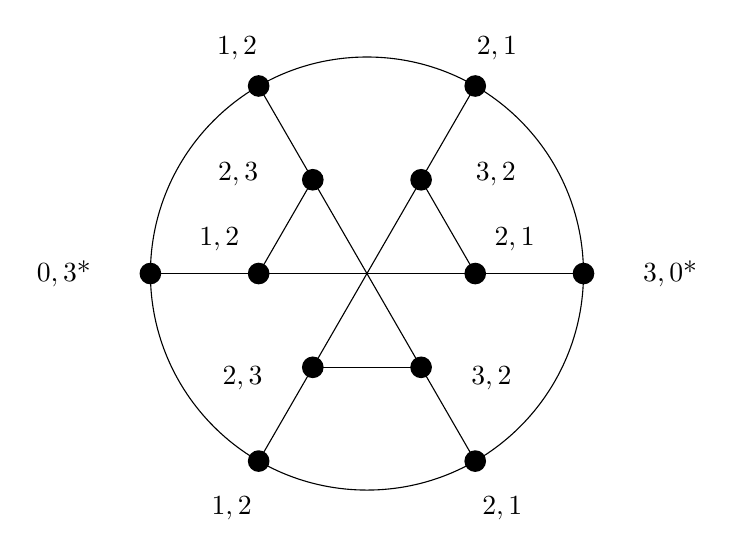
\begin{tikzpicture}[scale=2.75]
				\draw[white] (225:1.6) rectangle (45:1.6);
				\foreach \x/\y in
				{D/60, F/180, J/300}{
					\coordinate(\x) at (\y:0.5);
					\fill (\x) circle (0.5mm);
				}
				\foreach \x/\y in
				{C/120, G/0, I/240}{
					\coordinate(\x) at (\y:0.5);
					\fill (\x) circle (0.5mm);
				}
				
				
				\foreach \x/\y in
				{H/0, B/60, A/120, E/180, K/240, L/300}{
					\coordinate(\x) at (\y:1);
					\fill (\x) circle (0.5mm);
				}
				
				% inner ring (right)
				\node at (13:0.7){$2,1$}; % G/0
				\node at (37.5:0.75){$3,2$}; % D/60
				\node at (320:0.75){$3,2$}; % J/300
				
				% inner ring (left)
				\node at (142.5:0.75){$2,3$}; % C/135
				\node at (167:0.7){$1,2$}; % F/180
				\node at (220:0.75){$2,3$}; % I/225
				
				% outer ring
				\node at (0:1.4){$3,0$*}; % H/0
				\node at (120:1.2){$1,2$}; % A/120
				\node at (60:1.2){$2,1$}; % B/60
				\node at (180:1.4){$0,3$*}; % E/180
				\node at (240:1.25){$1,2$}; % K/240
				\node at (300:1.25){$2,1$}; % L/300
				
				\foreach \x/\y in 
				{I/D,D/B,H/G,G/F,F/C,C/J,J/I,A/C,E/F,D/G,K/I,L/J}{
					\draw (\x)--(\y);
				}
				\draw circle (1);
			\end{tikzpicture}
		\end{center}
		This provides the chaser with 6 different distances, $(0,3),(3,0),(1,2),(2,1),(2,3)$ and $(3,2)$. Consider the fact that $(0,3)$ and $(3,0)$ are unique distances. It follows then that if the runner is on vertices $E$ or $H$, it must be the case that the runner will be caught. This leaves the chaser with 4 different non-unique distances of $(1,2),(2,1),(2,3),$ and $(3,2)$. We will now proceed by cases.
		
		\textbf{Case 1:} Consider the case where the chaser has been returned a distance of $(1,2)$ from the first probes on vertices $E$ and $H$. Then the runner must be at one of the vertices $A,F$, or $K$. Recall that the runner cannot move on to $E$ or $H$ because of the no backtracking condition. It follows then that the runner has the ability to move to any of the neighboring vertices $B,C,G,I,L$. Thus, the runner could potentially be located at any of the vertices $A,B,C,F,G,I,K,L$.
		
		The chaser should now probe vertices $F$ and $K$.
		\begin{center}
			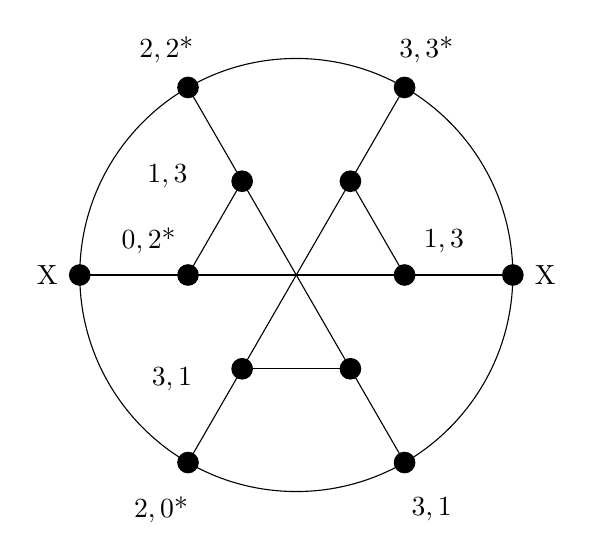
\begin{tikzpicture}[scale=2.75]
				\draw[white] (225:1.6) rectangle (45:1.6);
				\foreach \x/\y in
				{D/60, F/180, J/300}{
					\coordinate(\x) at (\y:0.5);
					\fill (\x) circle (0.5mm);
				}
				\foreach \x/\y in
				{C/120, G/0, I/240}{
					\coordinate(\x) at (\y:0.5);
					\fill (\x) circle (0.5mm);
				}
				
				
				\foreach \x/\y in
				{H/0, B/60, A/120, E/180, K/240, L/300}{
					\coordinate(\x) at (\y:1);
					\fill (\x) circle (0.5mm);
				}
				
				% inner ring (right)
				\node at (13:0.7){$1,3$}; % G/0
				
				% inner ring (left)
				\node at (142.5:0.75){$1,3$}; % C/135
				\node at (167:0.7){$0,2$*}; % F/180
				\node at (220:0.75){$3,1$}; % I/225
				
				% outer ring
				\node at (120:1.2){$2,2$*}; % A/120
				\node at (60:1.2){$3,3$*}; % B/60
				\node at (180:1.15){X}; % E/180
				\node at (0:1.15){X}; % H/0
				\node at (240:1.25){$2,0$*}; % K/240
				\node at (300:1.25){$3,1$}; % L/300
				
				\foreach \x/\y in 
				{I/D,D/B,H/G,G/F,F/C,C/J,J/I,A/C,E/F,D/G,K/I,L/J}{
					\draw (\x)--(\y);
				}
				\draw circle (1);
			\end{tikzpicture}
		\end{center}
		
		This again provides the chaser with 6 different distances, $(2,2),(3,3),(1,3),(0,2),(3,1),$ and $(2,0)$. Consider the fact that $(2,2),(3,3),(0,2)$ and $(2,0)$ are unique distances. It follows then that if the runner is on vertices $A,B,F,$ or $K$, it must be the case that the runner will be caught. This leaves the chaser with 2 different non-unique distances of $(1,3)$ and $(3,1)$. We will again proceed by cases.
		
		\textbf{Subcase 1.1:} Consider the case where the chaser has been returned a distance of $(1,3)$ from probing vertices $F$ and $K$. Then the runner must either be on vertex $C$ or vertex $G$. Recall that the runner cannot move on to vertex $F$ or vertex $K$ because of the no backtracking condition. It follows then that the runner has the ability to move to any of the neighboring vertices $A,D,F,H,J$. Thus, the runner could potentially be located at any of the vertices $A,C,D,G,H,J$.
		
		The chaser should now probe vertices $C$ and $I$.
		\begin{center}
			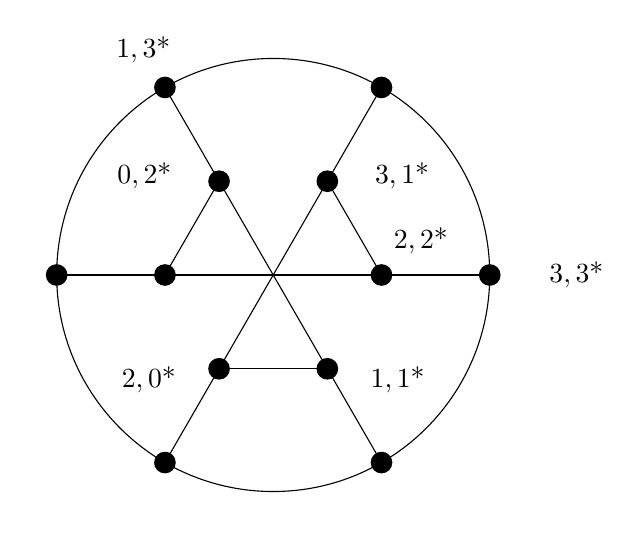
\begin{tikzpicture}[scale=2.75]
				\draw[white] (225:1.6) rectangle (45:1.6);
				\foreach \x/\y in
				{D/60, F/180, J/300}{
					\coordinate(\x) at (\y:0.5);
					\fill (\x) circle (0.5mm);
				}
				\foreach \x/\y in
				{C/120, G/0, I/240}{
					\coordinate(\x) at (\y:0.5);
					\fill (\x) circle (0.5mm);
				}
				
				
				\foreach \x/\y in
				{H/0, B/60, A/120, E/180, K/240, L/300}{
					\coordinate(\x) at (\y:1);
					\fill (\x) circle (0.5mm);
				}
				
				% inner ring (right)
				\node at (13:0.7){$2,2$*}; % G/0
				\node at (37.5:0.75){$3,1$*}; % D/60
				\node at (320:0.75){$1,1$*}; % J/300
				
				% inner ring (left)
				\node at (142.5:0.75){$0,2$*}; % C/135
				\node at (220:0.75){$2,0$*}; % I/225
				
				% outer ring
				\node at (0:1.4){$3,3$*}; % H/0
				\node at (120:1.2){$1,3$*}; % A/120
				
				\foreach \x/\y in 
				{I/D,D/B,H/G,G/F,F/C,C/J,J/I,A/C,E/F,D/G,K/I,L/J}{
					\draw (\x)--(\y);
				}
				\draw circle (1);
			\end{tikzpicture}
		\end{center}
		
		This provides the chaser with 7 different distances, $(1,3),(0,2),(3,1),(2,2),(3,3),(2,0)$, and $(1,1)$. Consider the fact that these are all unique distances. It follows then that the runner must be caught.
		
		\textbf{Subcase 1.2:} Consider the case where the chaser has been returned a distance of $(3,1)$ from probing vertices $F$ and $K$. Then the runner must either be on vertex $I$ or vertex $L$. Recall that the runner cannot move on to vertex $F$ or vertex $K$ because of the no backtracking condition. It follows then that the runner has the ability to move to any of the neighboring vertices $D,H,J$. Thus, the runner could potentially be located at any of the vertices $D,H,I,J,L$.
		
		The chaser should now probe vertices $D$ and $J$.
		\begin{center}
			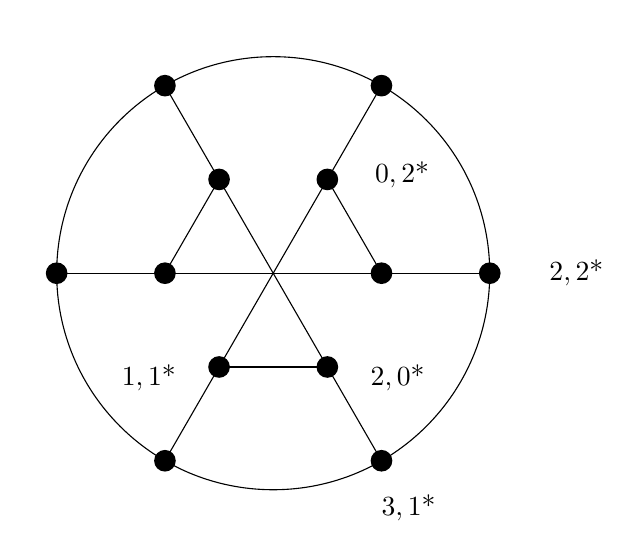
\begin{tikzpicture}[scale=2.75]
				\draw[white] (225:1.6) rectangle (45:1.6);
				\foreach \x/\y in
				{D/60, F/180, J/300}{
					\coordinate(\x) at (\y:0.5);
					\fill (\x) circle (0.5mm);
				}
				\foreach \x/\y in
				{C/120, G/0, I/240}{
					\coordinate(\x) at (\y:0.5);
					\fill (\x) circle (0.5mm);
				}
				
				
				\foreach \x/\y in
				{H/0, B/60, A/120, E/180, K/240, L/300}{
					\coordinate(\x) at (\y:1);
					\fill (\x) circle (0.5mm);
				}
				
				% inner ring (right)
				\node at (37.5:0.75){$0,2$*}; % D/60
				\node at (320:0.75){$2,0$*}; % J/300
				
				% inner ring (left)
				\node at (220:0.75){$1,1$*}; % I/225
				
				% outer ring
				\node at (0:1.4){$2,2$*}; % H/0
				\node at (300:1.25){$3,1$*}; % L/300
				
				\foreach \x/\y in 
				{I/D,D/B,H/G,G/F,F/C,C/J,J/I,A/C,E/F,D/G,K/I,L/J}{
					\draw (\x)--(\y);
				}
				\draw circle (1);
			\end{tikzpicture}
		\end{center}
		
		This provides the chaser with 5 different distances, $(0,2),(2,2),(1,1),(2,0)$ and $(3,1)$. Consider the fact that these are all unique distances. It follows then that the runner must be caught.
		
		\textbf{Case 2:} Consider the case where the chaser has been returned a distance of $(2,1)$ from the first probes on vertices $E$ and $H$. Then the runner must be at one of the vertices $B,G$, or $L$. Recall that the runner cannot move on to $E$ or $H$ because of the no backtracking condition. It follows then that the runner then has the ability to move to any of the neighboring vertices $A,D,F,J,K$. Thus, the runner could potentially be located at any of the vertices $A,B,D,F,G,J,K,L$.
		
		The chaser should now probe vertices $G$ and $L$.
		\begin{center}
			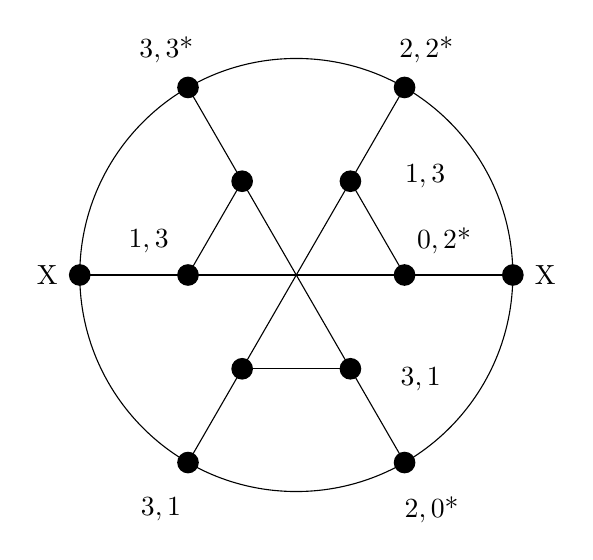
\begin{tikzpicture}[scale=2.75]
				\draw[white] (225:1.6) rectangle (45:1.6);
				\foreach \x/\y in
				{D/60, F/180, J/300}{
					\coordinate(\x) at (\y:0.5);
					\fill (\x) circle (0.5mm);
				}
				\foreach \x/\y in
				{C/120, G/0, I/240}{
					\coordinate(\x) at (\y:0.5);
					\fill (\x) circle (0.5mm);
				}
				
				
				\foreach \x/\y in
				{H/0, B/60, A/120, E/180, K/240, L/300}{
					\coordinate(\x) at (\y:1);
					\fill (\x) circle (0.5mm);
				}
				
				% inner ring (right)
				\node at (13:0.7){$0,2$*}; % G/0
				\node at (37.5:0.75){$1,3$}; % D/60
				\node at (320:0.75){$3,1$}; % J/300
				
				% inner ring (left)
				\node at (167:0.7){$1,3$}; % F/180
				
				% outer ring
				\node at (0:1.15){X}; % H/0
				\node at (120:1.2){$3,3$*}; % A/120
				\node at (60:1.2){$2,2$*}; % B/60
				\node at (180:1.15){X}; % E/180
				\node at (240:1.25){$3,1$}; % K/240
				\node at (300:1.25){$2,0$*}; % L/300
				
				\foreach \x/\y in 
				{I/D,D/B,H/G,G/F,F/C,C/J,J/I,A/C,E/F,D/G,K/I,L/J}{
					\draw (\x)--(\y);
				}
				\draw circle (1);
			\end{tikzpicture}
		\end{center}
		This again provides the chaser with 6 different distances, $(3,3),(2,2),(1,3),(0,2),(3,1),$ and $(2,0)$. Consider the fact that $(3,3),(2,2),(0,2)$, and $(2,0)$ are unique distances. It follows then that if the runner is on vertices $A,B,G,$ or $L$, it must be the case that the runner will be caught. This leaves the chaser with 2 different non-unique distances of $(1,3)$ and $(3,1)$. We will again proceed by cases.
		
		\textbf{Subcase 2.1} Consider the case where the chaser has been returned a distance of $(1,3)$ from probing vertices $G$ and $L$. Then the runner must either be on vertex $D$ or vertex $F$. Recall that the runner cannot move on to vertex $G$ or vertex $L$ because of the no backtracking condition. It follows then that the runner has the ability to move to any of the neighboring vertices $B,C,E,I$. Thus, the runner could potentially be located at any of the vertices $B,C,D,E,F,I$.
		
		The chaser should now probe $F$ and $K$.
		\begin{center}
			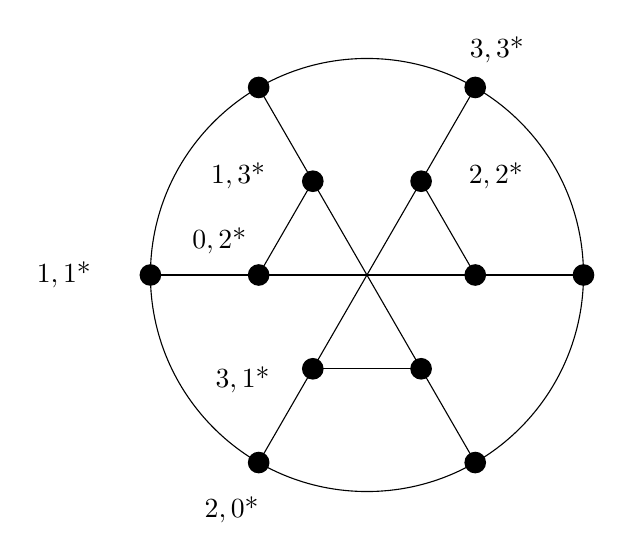
\begin{tikzpicture}[scale=2.75]
				\draw[white] (225:1.6) rectangle (45:1.6);
				\foreach \x/\y in
				{D/60, F/180, J/300}{
					\coordinate(\x) at (\y:0.5);
					\fill (\x) circle (0.5mm);
				}
				\foreach \x/\y in
				{C/120, G/0, I/240}{
					\coordinate(\x) at (\y:0.5);
					\fill (\x) circle (0.5mm);
				}
				
				
				\foreach \x/\y in
				{H/0, B/60, A/120, E/180, K/240, L/300}{
					\coordinate(\x) at (\y:1);
					\fill (\x) circle (0.5mm);
				}
				
				% inner ring (right)
				\node at (37.5:0.75){$2,2$*}; % D/60
				
				% inner ring (left)
				\node at (142.5:0.75){$1,3$*}; % C/135
				\node at (167:0.7){$0,2$*}; % F/180
				\node at (220:0.75){$3,1$*}; % I/225
				
				% outer ring
				\node at (60:1.2){$3,3$*}; % B/60
				\node at (180:1.4){$1,1$*}; % E/180
				\node at (240:1.25){$2,0$*}; % K/240
				
				\foreach \x/\y in 
				{I/D,D/B,H/G,G/F,F/C,C/J,J/I,A/C,E/F,D/G,K/I,L/J}{
					\draw (\x)--(\y);
				}
				\draw circle (1);
			\end{tikzpicture}
		\end{center}
		This provides the chaser with 7 different distances, $(3,3),(1,3),(2,2),(1,1),(0,2),(3,1),$ and $(2,0)$. Consider the fact that these are all unique distances. It follows then that the runner must be caught.
		
		\textbf{Subcase 2.2} Consider the case where the chaser has returned a distance of $(3,1)$ from probing vertices $G$ and $L$. Then the runner must either be on vertex $J$ or vertex $K$. Recall that the runner cannot move on to vertex $G$ or vertex $L$ because of the no backtracking condition. It follows then that the runner has the ability to move to any of the neighboring vertices, $C,E,I$. Thus, the runner could potentially be located at any of the vertices, $C,E,I,J,K$.
		
		The chaser should now probe vertices $C$ and $I$.
		\begin{center}
			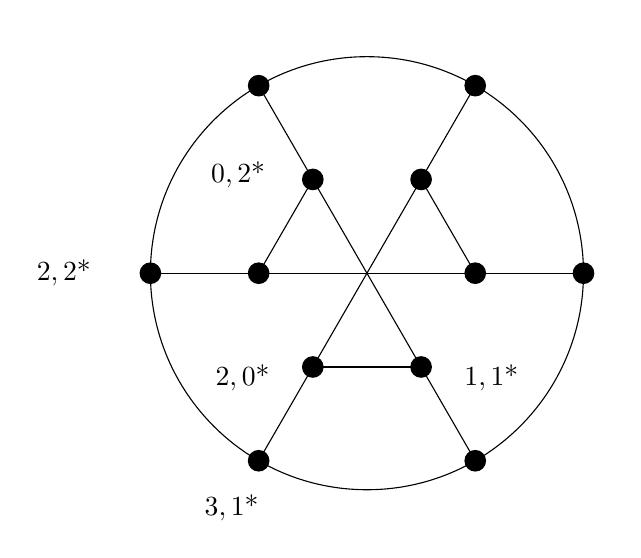
\begin{tikzpicture}[scale=2.75]
				\draw[white] (225:1.6) rectangle (45:1.6);
				\foreach \x/\y in
				{D/60, F/180, J/300}{
					\coordinate(\x) at (\y:0.5);
					\fill (\x) circle (0.5mm);
				}
				\foreach \x/\y in
				{C/120, G/0, I/240}{
					\coordinate(\x) at (\y:0.5);
					\fill (\x) circle (0.5mm);
				}
				
				
				\foreach \x/\y in
				{H/0, B/60, A/120, E/180, K/240, L/300}{
					\coordinate(\x) at (\y:1);
					\fill (\x) circle (0.5mm);
				}
				
				% inner ring (right)
				\node at (320:0.75){$1,1$*}; % J/300
				
				% inner ring (left)
				\node at (142.5:0.75){$0,2$*}; % C/135
				\node at (220:0.75){$2,0$*}; % I/225
				
				% outer ring
				\node at (180:1.4){$2,2$*}; % E/180
				\node at (240:1.25){$3,1$*}; % K/240
				
				\foreach \x/\y in 
				{I/D,D/B,H/G,G/F,F/C,C/J,J/I,A/C,E/F,D/G,K/I,L/J}{
					\draw (\x)--(\y);
				}
				\draw circle (1);
			\end{tikzpicture}
		\end{center}
		This provides the chaser with 5 different distances, $(0,2),(2,2),(2,0),(1,1)$ and $(3,1)$. Consider the fact that these are all unique distances. It follows then that the runner must be caught.
		
		\textbf{Case 3:} Consider the case where the chaser has been returned a distance of $(2,3)$ from the first probes on vertices $E$ and $H$. Then the runner must be at vertex $C$ or vertex $I$. Recall that the runner cannot move on to $E$ or $H$ because of the no backtracking condition. It follows then that the runner then has the ability to move to any of the neighboring vertices $A,D,F,J,K$. Thus, the runner could potentially be located at any of the vertices $A,C,D,F,I,J,K,$.
		
		The chaser should now probe vertices $C$ and $L$.
		\begin{center}
			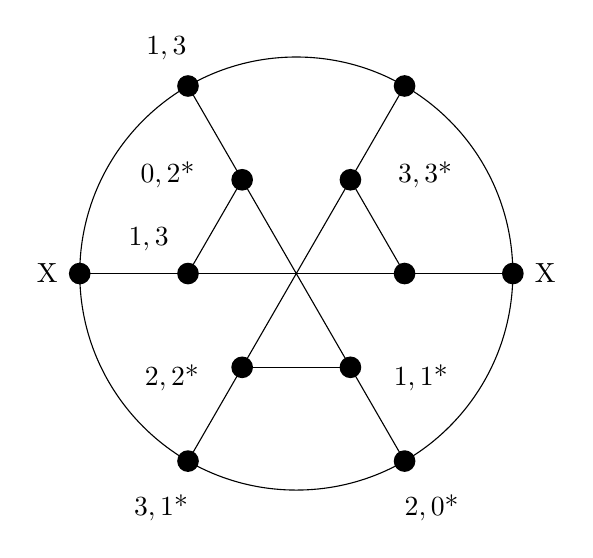
\begin{tikzpicture}[scale=2.75]
				\draw[white] (225:1.6) rectangle (45:1.6);
				\foreach \x/\y in
				{D/60, F/180, J/300}{
					\coordinate(\x) at (\y:0.5);
					\fill (\x) circle (0.5mm);
				}
				\foreach \x/\y in
				{C/120, G/0, I/240}{
					\coordinate(\x) at (\y:0.5);
					\fill (\x) circle (0.5mm);
				}
				
				
				\foreach \x/\y in
				{H/0, B/60, A/120, E/180, K/240, L/300}{
					\coordinate(\x) at (\y:1);
					\fill (\x) circle (0.5mm);
				}
				
				% inner ring (right)
				\node at (37.5:0.75){$3,3$*}; % D/60
				\node at (320:0.75){$1,1$*}; % J/300
				
				% inner ring (left)
				\node at (142.5:0.75){$0,2$*}; % C/135
				\node at (167:0.7){$1,3$}; % F/180
				\node at (220:0.75){$2,2$*}; % I/225
				
				% outer ring
				\node at (0:1.15){X}; % H/0
				\node at (120:1.2){$1,3$}; % A/120
				\node at (180:1.15){X}; % E/180
				\node at (240:1.25){$3,1$*}; % K/240
				\node at (300:1.25){$2,0$*}; % L/300
				
				\foreach \x/\y in 
				{I/D,D/B,H/G,G/F,F/C,C/J,J/I,A/C,E/F,D/G,K/I,L/J}{
					\draw (\x)--(\y);
				}
				\draw circle (1);
			\end{tikzpicture}
		\end{center}
		This provides the chaser with 7 different distances, $(1,3),(0,2),(3,3),(2,2), (1,1), (3,1)$ and $(2,0)$. Consider the fact that $(0,2),(3,3),(2,2),(1,1),(3,1)$, and $(2,0)$ are unique distances. It follows then that if the runner is on vertices $C,D,I,J,K$ or $L$, it must be the case that the runner will be caught. This leaves the chaser with 1 non-unique distance of $(1,3)$. Then the runner must either be on vertex $A$ or vertex $F$. Recall that the runner cannot move on to vertex $C$ or vertex $L$ because of the no backtracking condition. It follows then that the runner has the ability to move to any of the neighboring vertices $B,E,G$. Thus, the runner could potentially be located at any of the vertices $A,B,E,F,G$.
		
		The chaser should now probe vertices $A$ and $K$.
		\begin{center}
			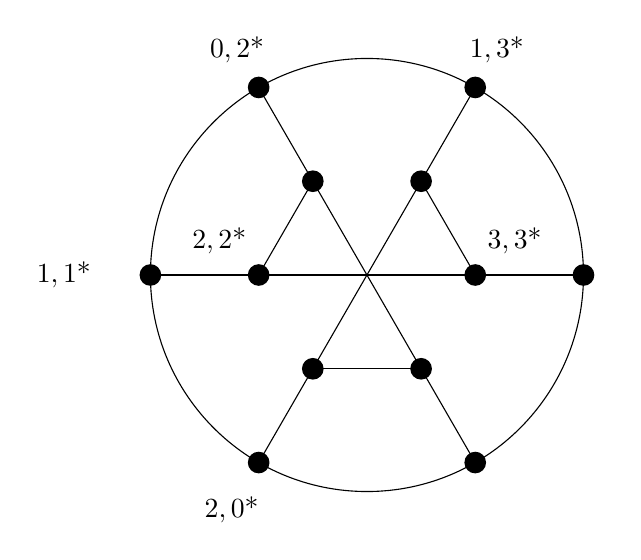
\begin{tikzpicture}[scale=2.75]
				\draw[white] (225:1.6) rectangle (45:1.6);
				\foreach \x/\y in
				{D/60, F/180, J/300}{
					\coordinate(\x) at (\y:0.5);
					\fill (\x) circle (0.5mm);
				}
				\foreach \x/\y in
				{C/120, G/0, I/240}{
					\coordinate(\x) at (\y:0.5);
					\fill (\x) circle (0.5mm);
				}
				
				
				\foreach \x/\y in
				{H/0, B/60, A/120, E/180, K/240, L/300}{
					\coordinate(\x) at (\y:1);
					\fill (\x) circle (0.5mm);
				}
				
				% inner ring (right)
				\node at (13:0.7){$3,3$*}; % G/0
				
				% inner ring (left)
				\node at (167:0.7){$2,2$*}; % F/180
				
				% outer ring
				\node at (120:1.2){$0,2$*}; % A/120
				\node at (60:1.2){$1,3$*}; % B/60
				\node at (180:1.4){$1,1$*}; % E/180
				\node at (240:1.25){$2,0$*}; % K/240
				
				\foreach \x/\y in 
				{I/D,D/B,H/G,G/F,F/C,C/J,J/I,A/C,E/F,D/G,K/I,L/J}{
					\draw (\x)--(\y);
				}
				\draw circle (1);
			\end{tikzpicture}
		\end{center}
		This provides the chaser with 6 different distances, $(0,2),(1,3),(1,1),(2,2),(3,3)$ and $(2,0)$. Consider the fact that these are all unique distances. It follows then that the runner must be caught.
		
		\textbf{Case 4:} Consider the case where the chaser has been returned a distance of $(3,2)$ from the first probes on vertices $E$ and $H$. Then the runner must be at vertex $D$ or vertex $J$. Recall that the runner cannot move on to $E$ or $H$ because of the no backtracking condition. It follows then that the runner then has the ability to move to any of the neighboring vertices $B,C,G,I,L$. Thus, the runner could potentially be located at any of the vertices $B,C,D,G,I,J,L$.
		
		The chaser should now probe vertices $D$ and $K$.
		\begin{center}
			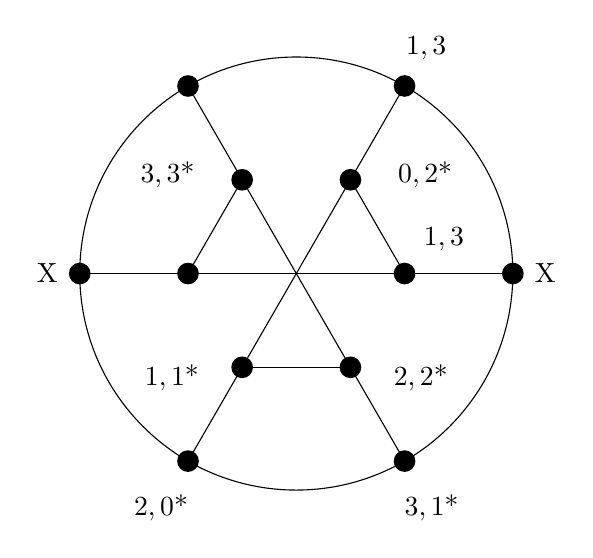
\begin{tikzpicture}[scale=2.75]
				\draw[white] (225:1.6) rectangle (45:1.6);
				\foreach \x/\y in
				{D/60, F/180, J/300}{
					\coordinate(\x) at (\y:0.5);
					\fill (\x) circle (0.5mm);
				}
				\foreach \x/\y in
				{C/120, G/0, I/240}{
					\coordinate(\x) at (\y:0.5);
					\fill (\x) circle (0.5mm);
				}
				
				
				\foreach \x/\y in
				{H/0, B/60, A/120, E/180, K/240, L/300}{
					\coordinate(\x) at (\y:1);
					\fill (\x) circle (0.5mm);
				}
				
				% inner ring (right)
				\node at (13:0.7){$1,3$}; % G/0
				\node at (37.5:0.75){$0,2$*}; % D/60
				\node at (320:0.75){$2,2$*}; % J/300
				
				% inner ring (left)
				\node at (142.5:0.75){$3,3$*}; % C/135
				\node at (220:0.75){$1,1$*}; % I/225
				
				% outer ring
				\node at (0:1.15){X}; % H/0
				\node at (60:1.2){$1,3$}; % B/60
				\node at (180:1.15){X}; % E/180
				\node at (240:1.25){$2,0$*}; % K/240
				\node at (300:1.25){$3,1$*}; % L/300
				
				\foreach \x/\y in 
				{I/D,D/B,H/G,G/F,F/C,C/J,J/I,A/C,E/F,D/G,K/I,L/J}{
					\draw (\x)--(\y);
				}
				\draw circle (1);
			\end{tikzpicture}
		\end{center}
		This provides the chaser with 7 different distances, $(1,3),(3,3),(0,2),(1,1), (2,2),(2,0)$ and $(3,1)$. Consider the fact that $(3,3),(0,2),(1,1),(2,2),(2,0)$, and $(3,1)$ are unique distances. It follows then that if the runner is on vertices $C,D,I,J,K$ or $L$, it must be the case that the runner will be caught. This leaves the chaser with 1 non-unique distance of $(1,3)$. Then the runner must either be on vertex $B$ or vertex $G$. Recall that the runner cannot move on to vertex $D$ or vertex $K$ because of the no backtracking condition. It follows then that the runner has the ability to move to any of the neighboring vertices $A,F,H$. Thus, the runner could potentially be located at any of the vertices $A,B,F,G,H$.
		
		The chaser should now probe vertices $A$ and $B$.
		\begin{center}
			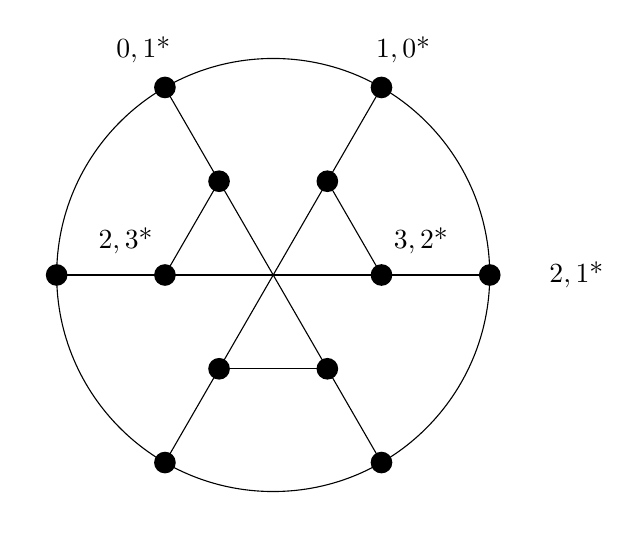
\begin{tikzpicture}[scale=2.75]
				\draw[white] (225:1.6) rectangle (45:1.6);
				\foreach \x/\y in
				{D/60, F/180, J/300}{
					\coordinate(\x) at (\y:0.5);
					\fill (\x) circle (0.5mm);
				}
				\foreach \x/\y in
				{C/120, G/0, I/240}{
					\coordinate(\x) at (\y:0.5);
					\fill (\x) circle (0.5mm);
				}
				
				
				\foreach \x/\y in
				{H/0, B/60, A/120, E/180, K/240, L/300}{
					\coordinate(\x) at (\y:1);
					\fill (\x) circle (0.5mm);
				}
				
				% inner ring (right)
				\node at (13:0.7){$3,2$*}; % G/0
				
				% inner ring (left)
				\node at (167:0.7){$2,3$*}; % F/180
				
				% outer ring
				\node at (0:1.4){$2,1$*}; % H/0
				\node at (120:1.2){$0,1$*}; % A/120
				\node at (60:1.2){$1,0$*}; % B/60
				
				\foreach \x/\y in 
				{I/D,D/B,H/G,G/F,F/C,C/J,J/I,A/C,E/F,D/G,K/I,L/J}{
					\draw (\x)--(\y);
				}
				\draw circle (1);
			\end{tikzpicture}
		\end{center}
		
		This provides the chaser with 6 different distances, $(0,1),(1,0),(2,3),(3,2)$ and $(2,1)$. Consider the fact that these are all unique distances. It follows then that the runner must be caught.
		
		Therefore, the Franklin Graph is locatable in 3 turns with 2 probes.
	\end{proof}
	\begin{clm}
		The Franklin Graph is not locatable with 1 probe.
	\end{clm}
	\begin{proof}
		\textbf{*insert Reilly's Balanced Bipartite 5 million condition theorem here*}.
		
		Therefore, the Franklin Graph is not locatable with 1 probe.
	\end{proof}
	% \begin{clm}
		% 	 The Franklin Graph is locatable with 3 probes.
		% \end{clm}
	% \begin{proof}
		% 	We begin by giving the chaser an optimal strategy to win in 3 turns with 3 probes. The chaser should begin by probing $C$, $G$, and $J$, then probe $A$, $D$, $H$. Lastly, probe $C$, $H$, and $J$.
		% \end{proof}
	\newpage
	
	\section{Watkins Snark}
	\begin{center}
		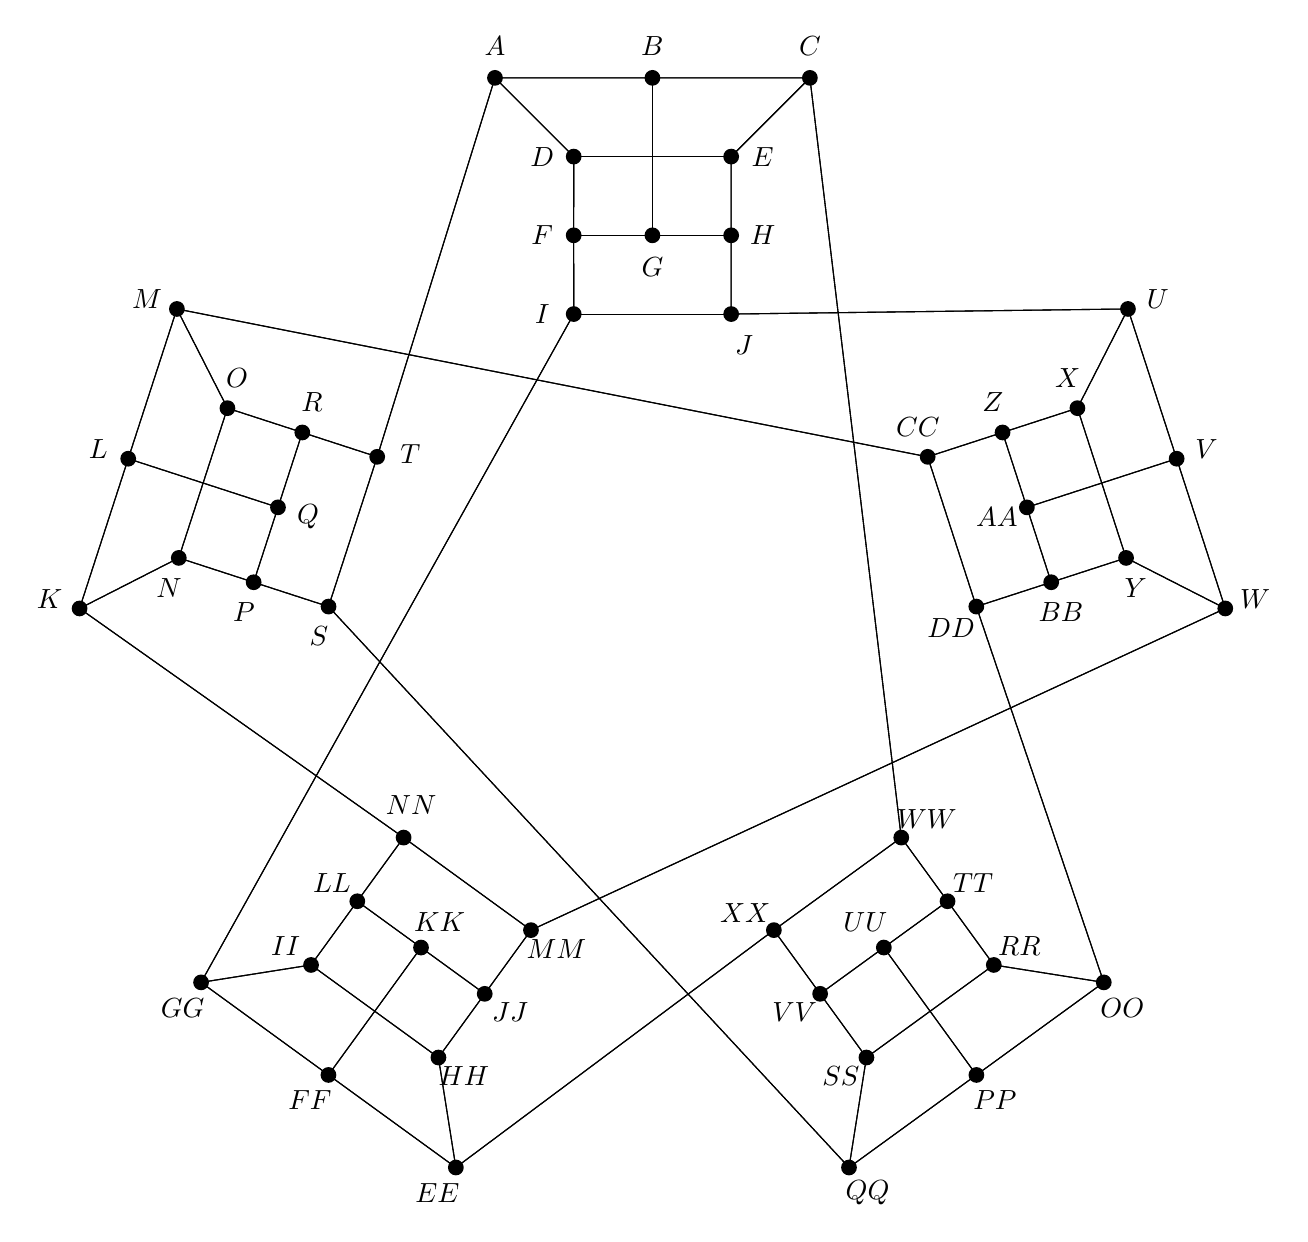
\begin{tikzpicture}[scale=1]
			% create 5 center points of each cluster
			\foreach \name/\angle in 
			{AA/18, G/90, Q/162, KK/234, UU/306}{
				\coordinate (\name) at (\angle:5);
				\fill (\name) circle (1mm);
				\node at (\angle:4.6){$\name$};
			}
			
			% what the heck has this mess become???
			\foreach \name/\offset/\leftlabels/\rightlabels/\toplabels in
			{G/0/{D/135/1.414, F/180/1, I/225/1.414}/{E/45/1.414, H/0/1}/{A/135/2.828, B/90/2, C/45/2.828},
				Q/72/{N/135/1.414, P/180/1, S/225/1.414}/{O/45/1.414, R/0/1}/{K/135/2.828, L/90/2, M/45/2.828},
				KK/144/{HH/135/1.414, JJ/180/1, MM/225/1.414}/{II/45/1.414, LL/0/1}/{EE/135/2.828, FF/90/2, GG/45/2.828},
				UU/216/{RR/135/1.414, TT/180/1, WW/225/1.414}/{SS/45/1.414, VV/0/1}/{OO/135/2.828, PP/90/2, QQ/45/2.828},
				AA/288/{X/135/1.414, Z/180/1, CC/225/1.414}/{Y/45/1.414, BB/0/1}/{U/135/2.828, V/90/2, W/45/2.828}}{
				\begin{scope}[shift={(\name)}]
					% left side
					\foreach \name/\angle/\distance in
					\leftlabels {
						\coordinate (\name) at ({\angle + \offset}:\distance);
						\fill (\name) circle (1mm);
						\begin{scope}[shift={(\name)}]
							\node at ({180 + \offset}:0.4){$\name$};
						\end{scope}
					}
					
					\foreach \name/\angle/\distance in
					\rightlabels {
						\coordinate (\name) at ({\angle + \offset}:\distance);
						\fill (\name) circle (1mm);
						\begin{scope}[shift={(\name)}]
							\node at ({0 + \offset}:0.4){$\name$};
						\end{scope}
					}
					
					\foreach \name/\angle/\distance in
					\toplabels {
						\coordinate (\name) at ({\angle + \offset}:\distance);
						\fill (\name) circle (1mm);
						\begin{scope}[shift={(\name)}]
							\node at ({90 + \offset}:0.4){$\name$};
						\end{scope}
					}
					
				\end{scope}
			}
			
			% the lower right labels in the above orientation will be in the way of an edge, create the lower right nodes and labels here
			\foreach \s/\n/\o/\d in {G/J/90/1.414, Q/T/162/1.414, KK/NN/234/1.414, UU/XX/306/1.414, AA/DD/18/1.414}{
				\begin{scope}[shift={(\s)}]
					\coordinate (\n) at ({315 - 90 + \o}:\d);
					\fill (\n) circle (1mm);
					\node at ({315 - 95 + \o}:1.814){$\n$};
				\end{scope}
			}
			
			% edges
			\foreach \x/\y in
			{A/B, A/D, A/T, B/A, B/C, B/G, C/B, C/E, C/WW, D/A, D/E, D/F, E/C, E/D, E/H, F/D, F/G, F/I, G/B, G/F, G/H, H/E, H/G, H/J, I/F, I/J, I/GG, J/H, J/I, J/U, K/L, K/N, K/NN, L/K, L/M, L/Q, M/L, M/O, M/CC, N/K, N/O, N/P, O/M, O/N, O/R, P/N, P/Q, P/S, Q/L, Q/P, Q/R, R/O, R/Q, R/T, S/P, S/T, S/QQ, T/A, T/R, T/S, U/J, U/V, U/X, V/U, V/W, V/AA, W/V, W/Y, W/MM, X/U, X/Y, X/Z, Y/W, Y/X, Y/BB, Z/X, Z/AA, Z/CC, AA/V, AA/Z, AA/BB, BB/Y, BB/AA, BB/DD, CC/M, CC/Z, CC/DD, DD/BB, DD/CC, DD/OO, EE/XX, EE/FF, EE/HH, FF/EE, FF/GG, FF/KK, GG/I, GG/FF, GG/II, HH/EE, HH/II, HH/JJ, II/GG, II/HH, II/LL, JJ/HH, JJ/KK, JJ/MM, KK/FF, KK/JJ, KK/LL, LL/II, LL/KK, LL/NN, MM/W, MM/JJ, MM/NN, NN/K, NN/LL, NN/MM, OO/DD, OO/PP, OO/RR, PP/OO, PP/QQ, PP/UU, QQ/S, QQ/PP, QQ/SS, RR/OO, RR/SS, RR/TT, SS/QQ, SS/RR, SS/VV, TT/RR, TT/UU, TT/WW, UU/PP, UU/TT, UU/VV, VV/SS, VV/UU, VV/XX, WW/C, WW/TT, WW/XX, XX/EE, XX/VV, XX/WW}{
				\draw (\x)--(\y);
			}
		\end{tikzpicture}
	\end{center}
	\begin{clm}
		The metric dimension of the Watkins snark is 3.
	\end{clm}
	\begin{proof}
		We begin by giving the chaser an optimal strategy to win in one turn with three probes. The chaser should probe vertices $A$, $U$, $NN$.
		
		This will result in unique distances for all vertices. Since every vertex has a unique distance, it must be the case that the runner is located. Since it is the case that the chaser is able to locate the runner in 1 turn with 3 probes, it logically follows that the metric dimension of the Watkins snark is less than or equal to 3.
		Thus, the metric dimension must be at most 3.
		
		We will now prove that the metric dimension cannot be 2. Reference Reilly's Cubic Theorem thingy.
		
		Since the metric dimension of the Watkins snark is less than or equal to 3 and the metric dimension of the Franklin graph cannot be 2, it must be the case where the metric dimension is greater than 2 and less than or equal to 3.
		
		Therefore, the metric dimension of the Watkins snark is 3.
	\end{proof}
	\begin{clm}
		The Watkins snark is locatable in 2 turns with 2 probes.
	\end{clm}
	\begin{proof}
		We begin by giving the chaser a strategy to win in 2 turns with 2 probes. The chaser should begin by probing the vertices $A$ and $FF$.
		
		This provides the chaser with 31 unique distances and 8 non-unique distances. The non-unique distances are $(2,4),(3,6),(4,4),(4,5),(5,4),(6,2),(6,5),$ and $(7,6)$. The runner is a vertex with a unique distance, then it must be the case that the runner will be caught. Thus, the runner can only be on a vertex with a non-unique distance. We will now proceed by cases.
		
		\textbf{Case 1:} Consider the case where the chaser has been returned a distance of $(2,4)$ from the first probes on vertices $A$ and $FF$. Then the runner must be at one of the vertices $C$ or $G$. Recall that the runner cannot move on to $A$ or $FF$ because of the no backtracking condition. It follows then that the runner has the ability to move to any of the neighboring vertices $B,E,F,H,WW$. Thus, the runner could potentially be located at any of the vertices $B,C,E,F,G,H,WW$.
		
		The chaser should now probe vertices $A$ and $GG$.
		
		This provides the chaser 7 different distances, . Consider the fact that these are all unique distances. It follows then that the runner must be caught.
		
		\textbf{Case 2:} Consider the case where the chaser has been returned a distance of $(3,6)$ from the first probes on vertices $A$ and $FF$. Then the runner must be at one of the vertices $O$, $Q$ or $P$. Recall that the runner cannot move on to $A$ or $FF$ because of the no backtracking condition. It follows then that the runner has the ability to move to any of the neighboring vertices $M,R,L,N,S$. Thus, the runner could potentially be located at any of the vertices $M,O,R,L,Q,N,P,S$.
		
		The chaser should now probe vertices $K$ and $QQ$.
		
		This provides the chaser 7 different distances, . Consider the fact that these are all unique distances. It follows then that the runner must be caught.
		
		\textbf{Case 3:} Consider the case where the chaser has been returned a distance of $(4,4)$ from the first probes on vertices $A$ and $FF$. Then the runner must be at one of the vertices $TT$ or $SS$. Recall that the runner cannot move on to $A$ or $FF$ because of the no backtracking condition. It follows then that the runner has the ability to move to any of the neighboring vertices $WW,VV,UU,RR,QQ$. Thus, the runner could potentially be located at any of the vertices $WW,VV,UU,TT,SS,RR,QQ$.
		
		The chaser should now probe vertices $C$ and $OO$.
		
		This provides the chaser 7 different distances, . Consider the fact that these are all unique distances. It follows then that the runner must be caught.
		
		\textbf{Case 4:} Consider the case where the chaser has been returned a distance of $(4,5)$ from the first probes on vertices $A$ and $FF$. Then the runner must be at one of the vertices $L$, $N$, or $PP$. Recall that the runner cannot move on to $A$ or $FF$ because of the no backtracking condition. It follows then that the runner has the ability to move to any of the neighboring vertices $M,O,Q,P,K,UU,QQ,OO$. Thus, the runner could potentially be located at any of the vertices $M,O,L,Q,N,P,K,UU,QQ,PP,OO$.
		
		The chaser should now probe vertices $A$ and $M$.
		
		This provides the chaser 11 different distances, . Consider the fact that these are all unique distances. It follows then that the runner must be caught.
		
		\textbf{Case 5:} Consider the case where the chaser has been returned a distance of $(5,4)$ from the first probes on vertices $A$ and $FF$. Then the runner must be at one of the vertices $U$, $K$, or $UU$. Recall that the runner cannot move on to $A$ or $FF$ because of the no backtracking condition. It follows then that the runner has the ability to move to any of the neighboring vertices $J,X,L,V,N,NN,VV,TT,PP$. Thus, the runner could potentially be located at any of the vertices $J,U,X,L,V,N,K,NN,VV,UU,TT,PP$.
		
		The chaser should now probe vertices $NN$ and $PP$.
		
		This provides the chaser 12 different distances, . Consider the fact that these are all unique distances. It follows then that the runner must be caught.
		
		\textbf{Case 6:} Consider the case where the chaser has been returned a distance of $(6,2)$ from the first probes on vertices $A$ and $FF$. Then the runner must be at one of the vertices $LL$ or $HH$. Recall that the runner cannot move on to $A$ or $FF$ because of the no backtracking condition. It follows then that the runner has the ability to move to any of the neighboring vertices $NN,KK,JJ,II,EE$. Thus, the runner could potentially be located at any of the vertices $NN,LL,KK,JJ,II,HH,EE$.
		
		The chaser should now probe vertices $W$ and $EE$.
		
		This provides the chaser 7 different distances, . Consider the fact that these are all unique distances. It follows then that the runner must be caught.
		
		\textbf{Case 7:} Consider the case where the chaser has been returned a distance of $(6,5)$ from the first probes on vertices $A$ and $FF$. Then the runner must be at one of the vertices $X$ or $V$. Recall that the runner cannot move on to $A$ or $FF$ because of the no backtracking condition. It follows then that the runner has the ability to move to any of the neighboring vertices $U,Z,AA,Y,W$. Thus, the runner could potentially be located at any of the vertices $U,Z,X,AA,V,Y,W$.
		
		The chaser should now probe vertices $M$ and $U$.
		
		This provides the chaser 7 different distances, . Consider the fact that these are all unique distances. It follows then that the runner must be caught.
		
		\textbf{Case 8:} Consider the case where the chaser has been returned a distance of $(7,6)$ from the first probes on vertices $A$ and $FF$. Then the runner must be at one of the vertices $AA$ or $BB$. Recall that the runner cannot move on to $A$ or $FF$ because of the no backtracking condition. It follows then that the runner has the ability to move to any of the neighboring vertices $Z,V,DD,Y$. Thus, the runner could potentially be located at any of the vertices $Z,AA,V,DD,BB,Y$.
		
		The chaser should now probe vertices $M$ and $U$.
		
		This provides the chaser 6 different distances, . Consider the fact that these are all unique distances. It follows then that the runner must be caught.
		
		Therefore, the Watkins snark is locatable in 2 turns with 2 probes.
	\end{proof}
	\begin{clm}
		The Watkins snark is not locatable with 1 probe.
	\end{clm}
	\begin{proof}
		It has a $C_5$, unfortunately a formal proof of that is not written up yet, but will be soon.
		
		\textbf{*insert $C_5$ formal proof/reference theorem here*}
		
		Therefore, the Watkins snark is not locatable with 1 probe.
	\end{proof}
\end{document}